%%% LaTeX Template: Article/Thesis/etc. with colored headings and special fonts
%%%
%%% Source: http://www.howtotex.com/
%%% Feel free to distribute this template, but please keep to referal to http://www.howtotex.com/ here.
%%% February 2011
%%%
%%% Modified May 2018 by CDM

%%%  Preamble
\documentclass[11pt,letterpaper]{article}
\usepackage[margin=1.0in]{geometry}
\usepackage[T1]{fontenc}
\usepackage[bitstream-charter]{mathdesign}
\usepackage[latin1]{inputenc}					
\usepackage{amsmath}						
\usepackage{xcolor}
\usepackage{cite}
\usepackage{hyphenat}
\usepackage{graphicx}
\usepackage{float}
\usepackage{subfigure}
\usepackage{sectsty}
\usepackage[compact]{titlesec} 
\usepackage[tablegrid]{vhistory}
\allsectionsfont{\color{accentcolor}\scshape\selectfont}

%%% Definitions
\definecolor{accentcolor}{rgb}{0.0,0.0,0.5} 
\newcommand{\teamname}{Team Name}
\newcommand{\productname}{Product Name}
\newcommand{\coursename}{CSE 4316: Senior Design I}
\newcommand{\semester}{Spring 2018}
\newcommand{\docname}{System Requirements Specification}
\newcommand{\department}{Department of Computer Science \& Engineering}
\newcommand{\university}{The University of Texas at Arlington}
\newcommand{\authors}{Alan Turing \\ Grace Hopper \\ John Von Neumann \\ Ada Lovelace \\ Charles Babbage}

%%% Headers and footers
\usepackage{fancyhdr}
	\pagestyle{fancy}						% Enabling the custom headers/footers
\usepackage{lastpage}	
	% Header (empty)
	\lhead{}
	\chead{}
	\rhead{}
	% Footer
	\lfoot{\footnotesize \teamname \ - \semester}
	\cfoot{}
	\rfoot{\footnotesize page \thepage\ of \pageref{LastPage}}	% "Page 1 of 2"
	\renewcommand{\headrulewidth}{0.0pt}
	\renewcommand{\footrulewidth}{0.4pt}

%%% Change the abstract environment
\usepackage[runin]{abstract}			% runin option for a run-in title
%\setlength\absleftindent{30pt}			% left margin
%\setlength\absrightindent{30pt}		% right margin
\abslabeldelim{\quad}	
\setlength{\abstitleskip}{-10pt}
\renewcommand{\abstractname}{}
\renewcommand{\abstracttextfont}{\color{accentcolor} \small \slshape}	% slanted text

%%% Start of the document
\begin{document}

%%% Cover sheet
{\centering \huge \color{accentcolor} \sc \textbf{\department \\ \university} \par}
\vspace{1 in}
{\centering \huge \color{accentcolor} \sc \textbf{\docname \\ \coursename \\ \semester} \par}
\vspace{0.5 in}
\begin{figure}[h!]
	\centering
   	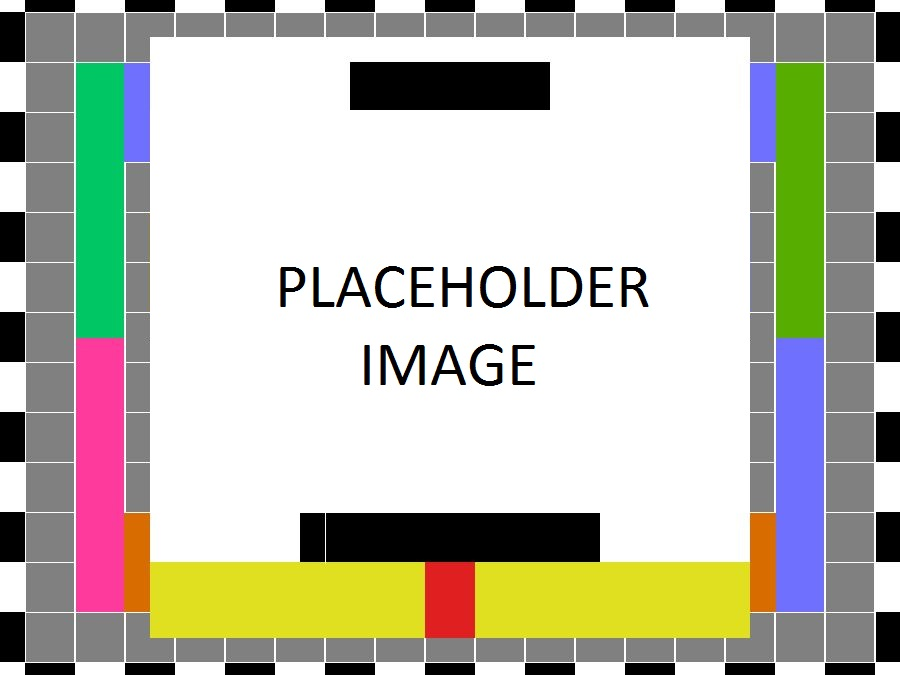
\includegraphics[width=0.60\textwidth]{images/test_image}
\end{figure}
\vspace{0.5 in}
{\centering \huge \color{accentcolor} \sc \textbf{\teamname \\ \productname} \par}
\vspace{0.5 in}
{\centering \large \sc \textbf{\authors} \par}
\newpage


%\vspace{1 in}
%\centerline{January 13th, 2012}
%\newpage

%%% Revision History
\begin{versionhistory}
  	\vhEntry{0.1}{10.01.2015}{GH}{document creation}
  	\vhEntry{0.2}{10.05.2015}{AT|GH}{complete draft}
  	\vhEntry{0.3}{10.12.2015}{AT|GH}{release candidate 1}
  	\vhEntry{1.0}{10.20.2015}{AT|GH|CB}{official release}
  	\vhEntry{1.1}{10.31.2015}{AL}{added customer change requests}
\end{versionhistory}
\newpage

%%% Table of contents
\setcounter{tocdepth}{3}
\tableofcontents
\newpage

%%% List of figures and tables (optional)
\listoffigures
%\listoftables
\newpage

\section{Product Concept}

\subsection{Purpose and Use}
The purpose of VoicePrint is to allow a user to control a 3D printer using voice commands. VoicePrint will be used to print small three-dimensional plastic objects on a 3D printer. 

\subsection{Intended Audience}
The intended audience for VoicePrint is consumers and hobbyists who own 3D printers and have Android smartphones. VoicePrint is a standalone product, but it does depend on the OctoPrint and Google Cloud Speech APIs.
\newpage
\section{Product Description}

\subsection{Features \& Functions}

\begin{figure}[h!]
	\centering
   	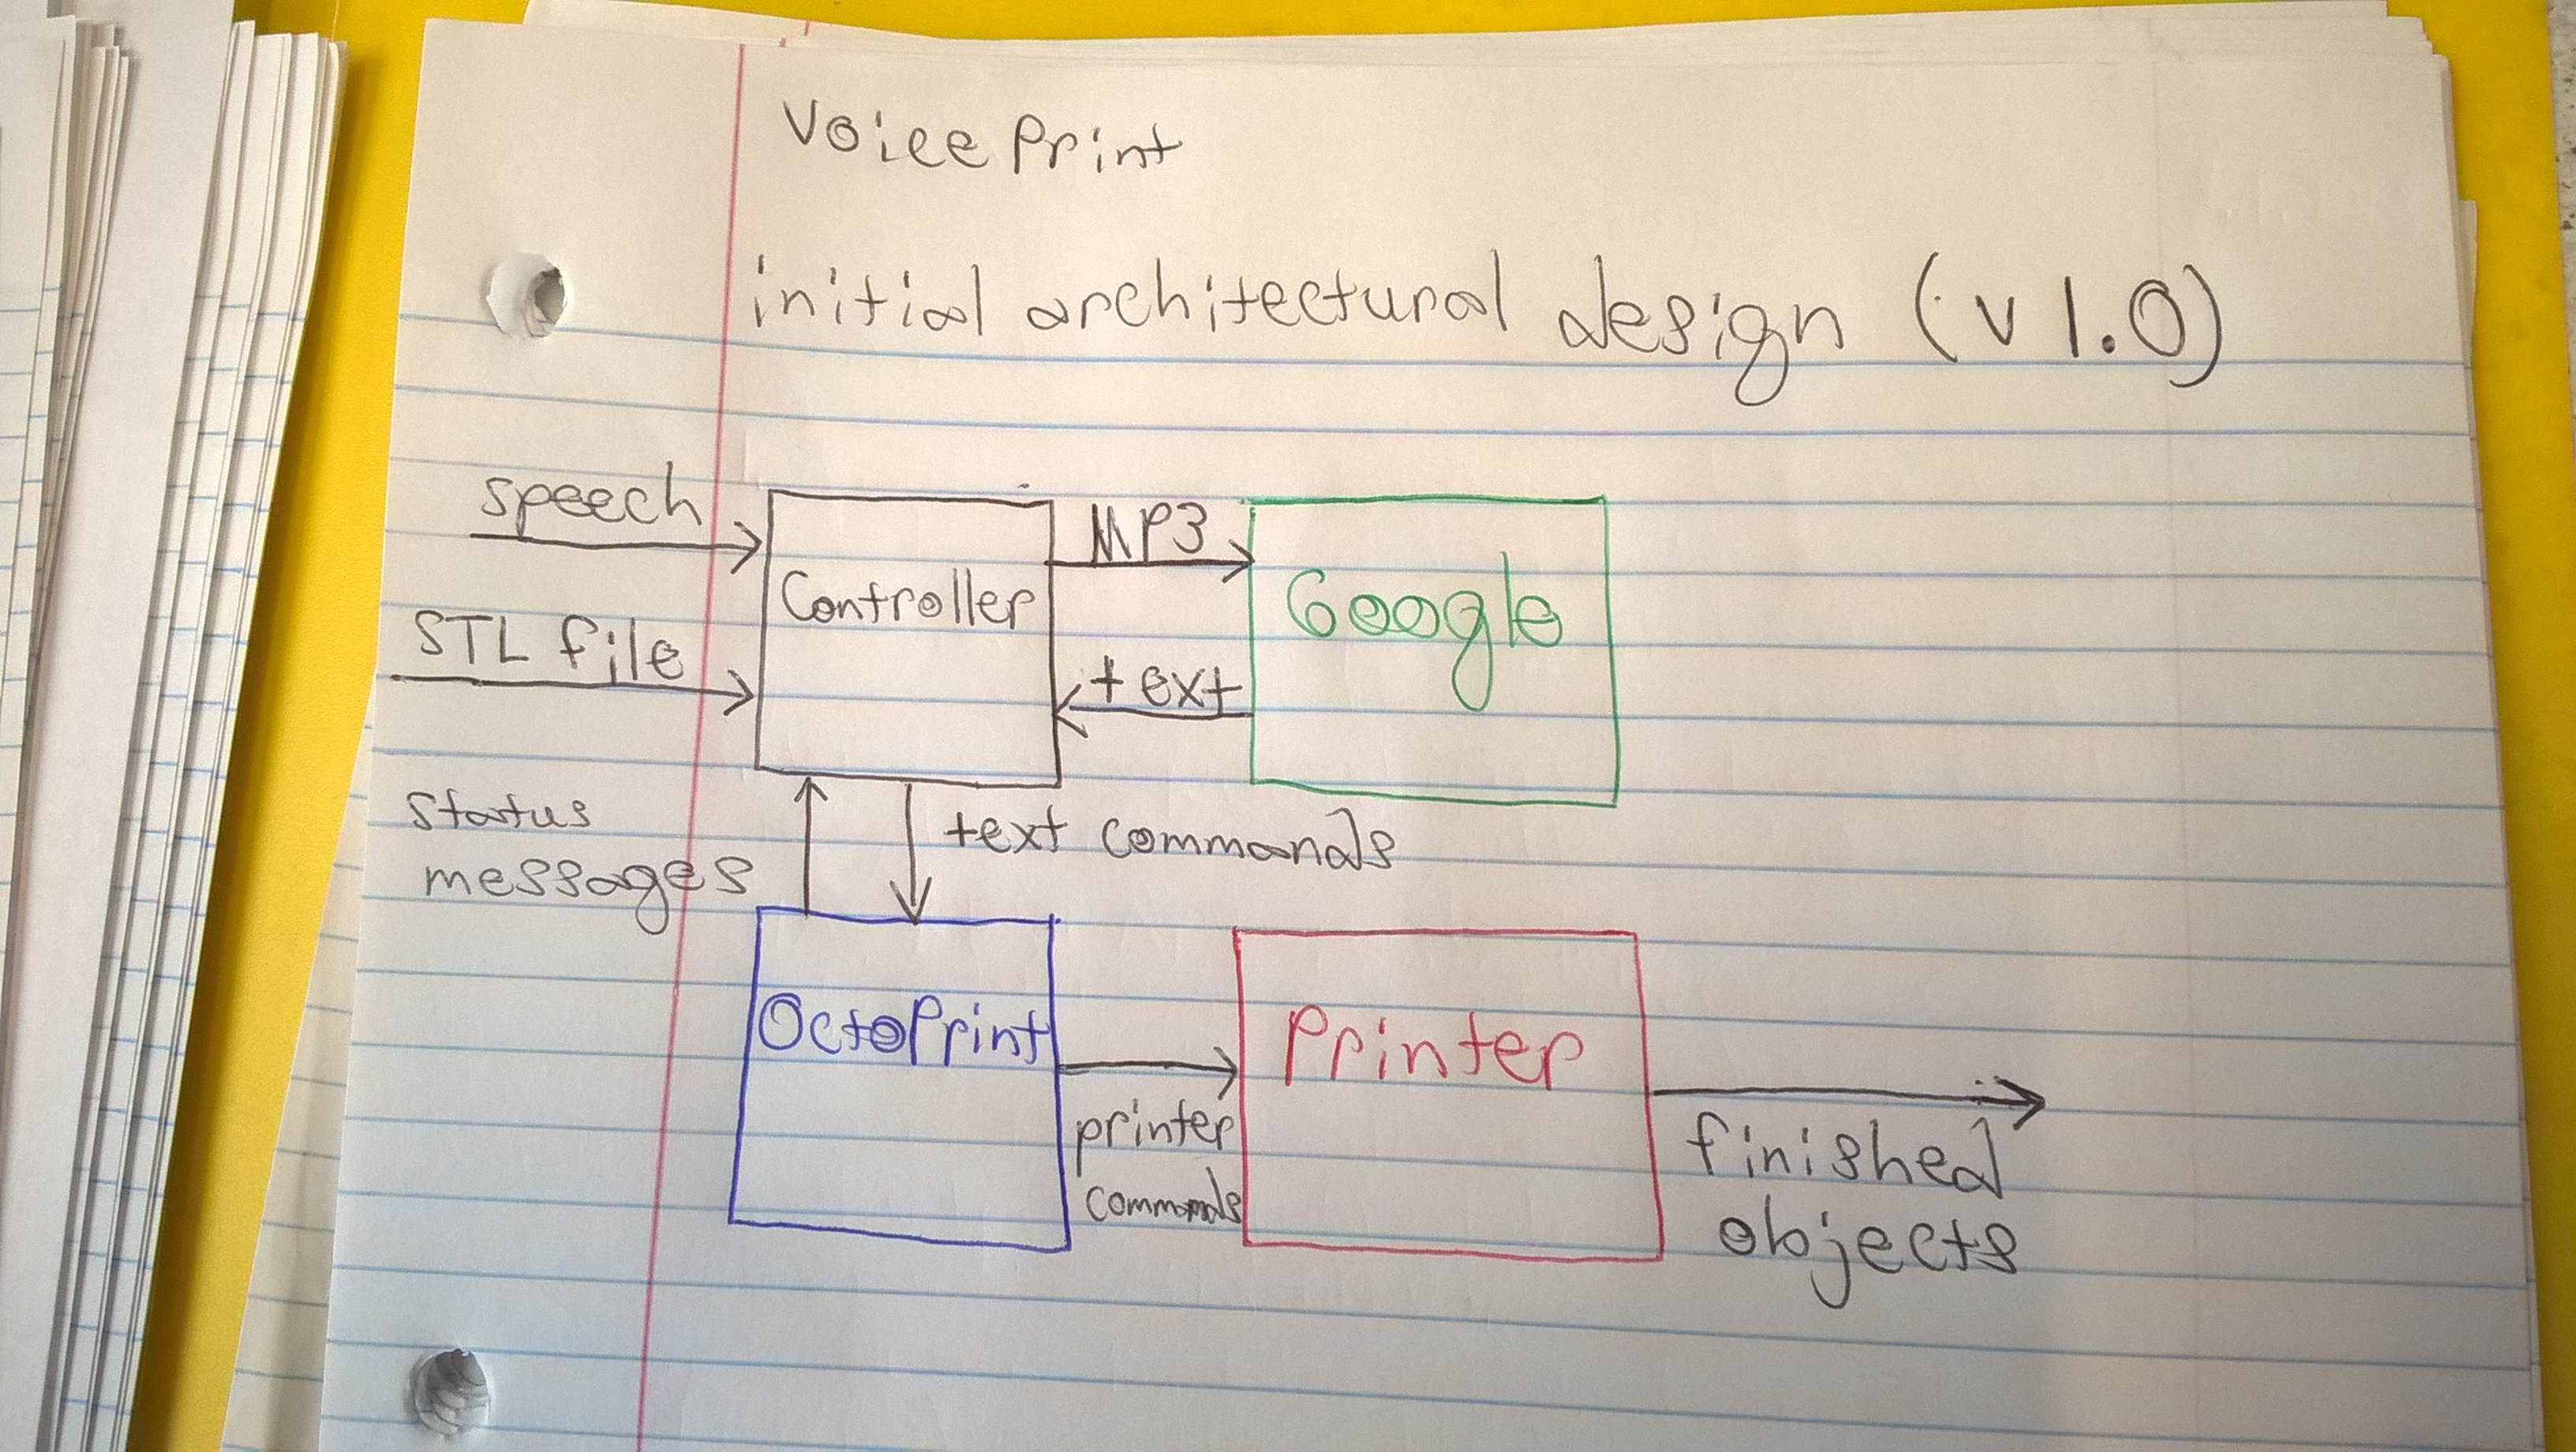
\includegraphics[width=0.60\textwidth]{images/architecture.jpg}
   	   	    \caption{VoicePrint app architecture}
\end{figure}

\begin{figure}[h!]
	\centering
   	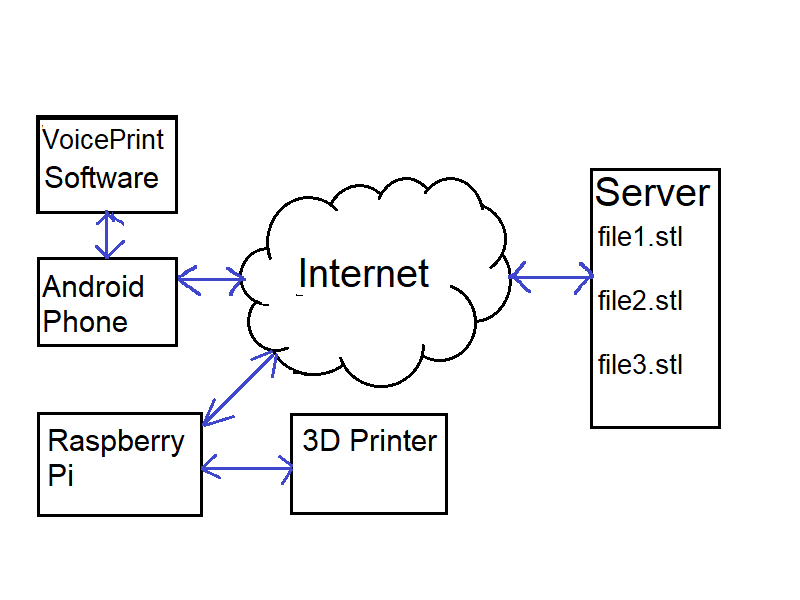
\includegraphics[width=0.60\textwidth]{images/vp1.png}
   	   	   	    \caption{System Architectural Framework}
\end{figure}

The VoicePrint system consists of five modules: the Controller (the VoicePrint Software), which is one or more Java classes that the senior design team will write; an Android smartphone (shown in Figure 2), Google Cloud Speech API (Google in Figure 1), which transcribes audio recorded by the phone into text; OctoPrint, an open-source API for controlling 3D printers; and the 3D printer itself (Printer in Figure 1). The phone records the user's voice commands and stores them for later processing, and it provides physical interaction with the user via the touchscreen. The Controller is responsible for taking user input, processing it, dispatching it to Google Cloud Speech and OctoPrint APIs and communicating with the external server (Google Cloud). Google Cloud (a.k.a. Server) transcribes audio into text and stores the STL files for the app. OctoPrint, in the form of OctoPi, running on a Raspberry Pi connected to the 3D printer, sends low-level commands to the printer to adjust its settings and print objects. The 3D printer is the physical hardware that prints the three-dimensional objects.

\subsection{External Inputs \& Outputs}

\begin{figure}[h!]
	\centering
   	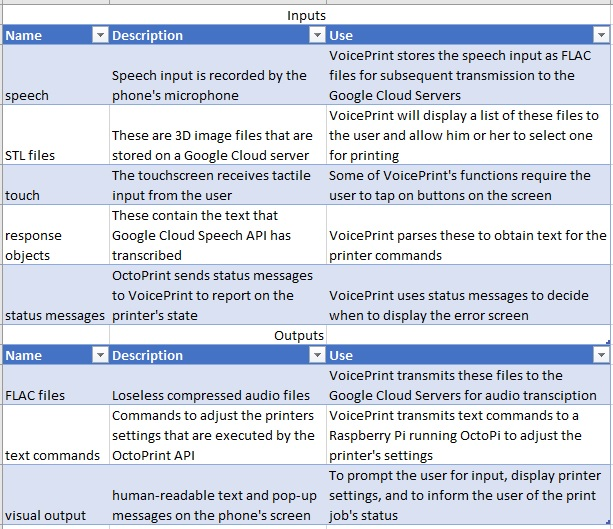
\includegraphics[width=1.00\textwidth]{images/table2.jpg}
   	\caption{Table of Critical Data Flows}
\end{figure}

\subsection{Product Interfaces}
Upon opening the app, VoicePrint will display a welcome message. Then it will display a list of files from which the user can choose. These files will be hosted on an external server (Server in Figure 1). VoicePrint will connect to this server over the Internet. The external server is a virtual machine in Google Cloud.

The VoicePrint user interface consists of 13 Android app activities (screens) that are displayed in roughly sequential order.
\newpage

\begin{figure}[h!]
	\centering
   	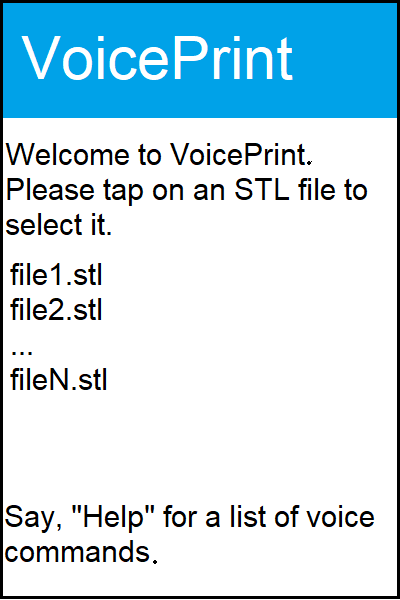
\includegraphics[width=0.60\textwidth]{images/Activity1.png}
   	\caption{Welcome Screen}
\end{figure}

The welcome screen allows a user to select an STL file that is stored on the external server.

\newpage

\begin{figure}[h!]
	\centering
   	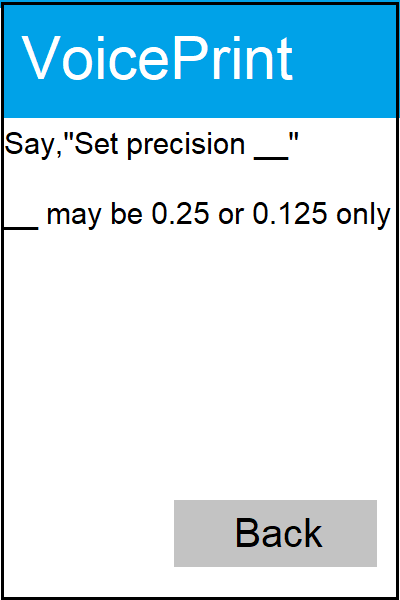
\includegraphics[width=0.60\textwidth]{images/Activity2.png}
   	\caption{Set Precision Screen}
\end{figure}

The set precision screen allows a user to set the precision for the 3D print job.

\newpage

\begin{figure}[h!]
	\centering
   	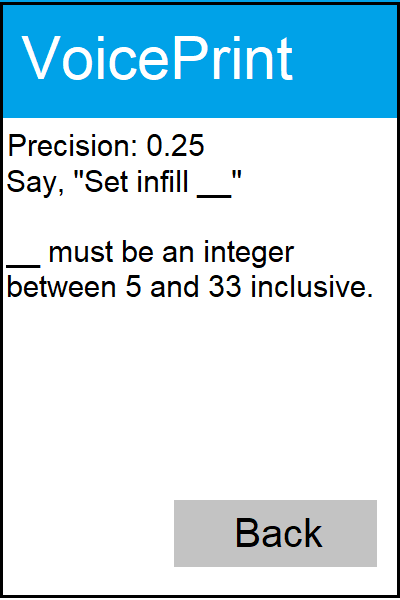
\includegraphics[width=0.60\textwidth]{images/Activity3.png}
   	\caption{Set Infill Screen}
\end{figure}

The set infill screen allows a user to set the infill for the 3D print job.

\newpage

\begin{figure}[h!]
	\centering
   	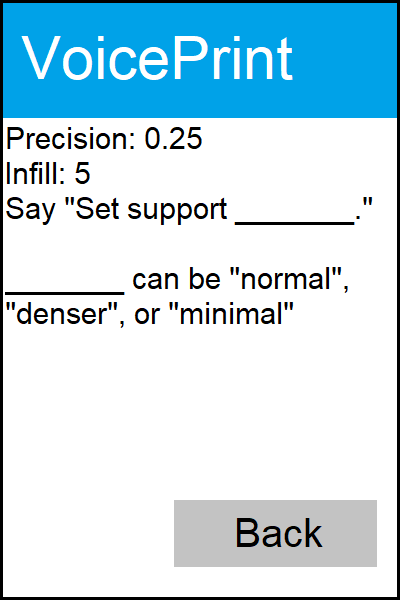
\includegraphics[width=0.60\textwidth]{images/Activity4.png}
   	\caption{Set Support Screen}
\end{figure}

The set support screen allows a user to set the support for the 3D print job.

\newpage

\begin{figure}[h!]
	\centering
   	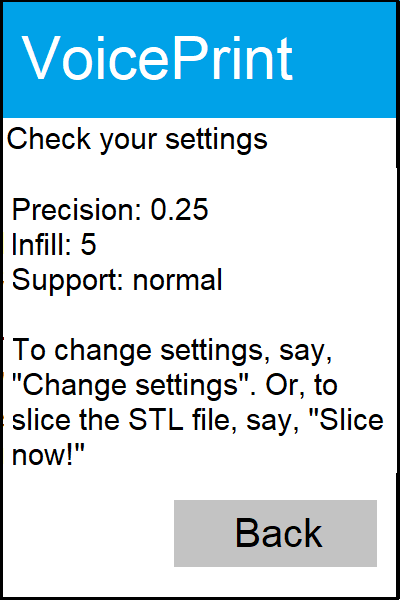
\includegraphics[width=0.60\textwidth]{images/Activity5.png}
   	\caption{Check Settings Screen}
\end{figure}

The check settings screen allows a user to review the settings that he or she has chosen and return to a previous step in order to change them, if necessary. Otherwise the user may order VoicePrint to slice the STL file into Gcode (low-level machine language instructions) for the 3D printer.

\newpage

\begin{figure}[h!]
	\centering
   	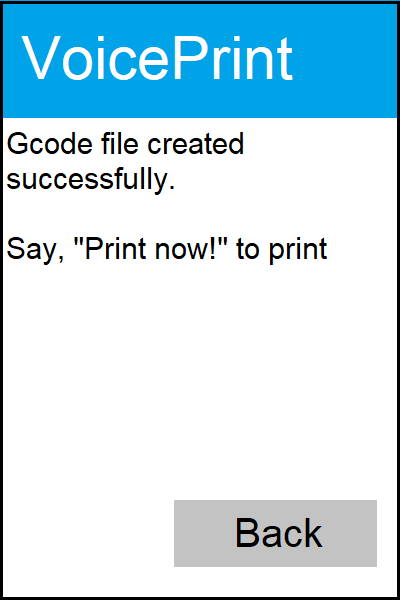
\includegraphics[width=0.60\textwidth]{images/Activity6a.png}
   	\caption{Ready-to-Print Screen}
\end{figure}

If VoicePrint slices the STL file successfully, then it will give the user the option to print it on the Ready-to-Print screen. If slicing failed, VoicePrint will go to the error activity.

\newpage

\begin{figure}[h!]
	\centering
   	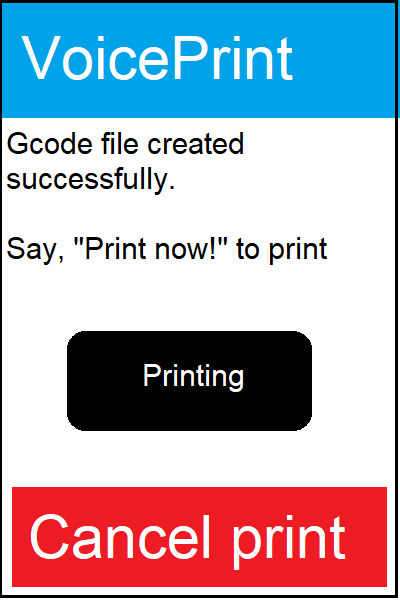
\includegraphics[width=0.60\textwidth]{images/Activity6b.png}
   	\caption{Now Printing Screen}
\end{figure}

When the user says, Print now! VoicePrint sends a command to the server to send the Gcode file to the Rasperry Pi which controls the 3D printer. The printer starts printing the object, and a pop-up message (called a toast in Android) is displayed on the device screen. This pop-up message says, Printing. While the printer is printing, a large red Cancel print button will also be displayed on the device screen. If he or she taps on this button, then VoicePrint will send a command to the Rasperry Pi to abort the print job and it will notify the user.

\newpage

\begin{figure}[h!]
	\centering
   	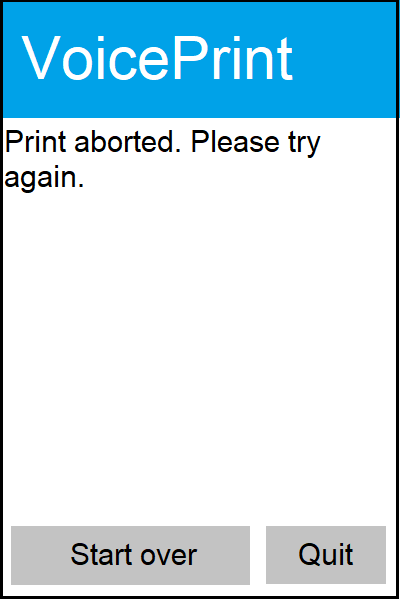
\includegraphics[width=0.60\textwidth]{images/Activity7.png}
   	\caption{Error Screen}
\end{figure}

If (1) there is an error in slicing STL file, (2) there is an error in printing the Gcode file , or (3) the user taps the Cancel print button on the Now Printing Screen, then VoicePrint will display the error screen. The error screen gives the user two options: Start Over or Quit. Start Over returns to the welcome screen. Quit closes the app.

\newpage

\begin{figure}[h!]
	\centering
   	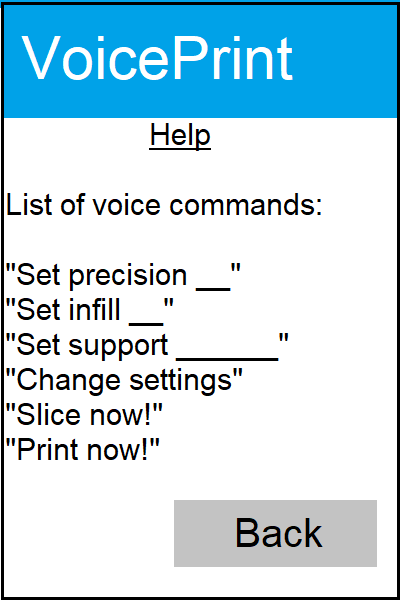
\includegraphics[width=0.60\textwidth]{images/ActivityHelp.png}
   	\caption{Help Screen}
\end{figure}

The help screen displays a list of acceptable voice commands which the app recognizes. It may be accessed at any time by saying Help.


\newpage
\section{Customer Requirements}
Include a header paragraph specific to your product here. Customer requirements are those required features and functions specified for and by the intended audience for this product. This section establishes, clearly and concisely, the "look and feel" of the product, what each potential end-user should expect the product do and/or not do. Each requirement specified in this section is associated with a specific customer need that will be satisfied. In general Customer Requirements are the directly observable features and functions of the product that will be encountered by its users. Requirements specified in this section are created with, and must not be changed without, specific agreement of the intended customer/user/sponsor.

\subsection{Android Application}
\subsubsection{Description}
Voiceprint will be an android application.
\subsubsection{Source}
??
\subsubsection{Constraints}
No iOS application will be produced due to time constraints and lack of resources.
\subsubsection{Standards}
The application will need to adhere to Google's term of service on the Google Play Store.
\subsubsection{Priority}
Critical
\subsection{Google Cloud API}
\subsubsection{Description}
The voiceprint app will use the Google Cloud API for voice command recognition.
\subsubsection{Source}
???
\subsubsection{Constraints}
The technology involved in speech recognition will be constrained by Google's speech API ability. 
\subsubsection{Standards}
Voice commands will be limited to the standards of Google's Cloud API for speech recognition. 
\subsubsection{Priority}
Critical
\subsection{User Friendly Interface}
\subsubsection{Description}
The application will feature an user friendly interface.
\subsubsection{Source}
???
\subsubsection{Constraints}
Some features may need some degree of technicality. 
\subsubsection{Standards}
The interface will need to meet Google Play's standards.
\subsubsection{Priority}
High
\subsection{STL files stored on external server}
\subsubsection{Description}
A user can select and print from an STL file stored on an external server.
\subsubsection{Source}
Peter Severynen
\subsubsection{Constraints}
External server use may be limited due to authentication or user permission.
\subsubsection{Standards}
The app will need to adhere to the standards involving file access from various external servers owned by different companies.
\subsubsection{Priority}
High
\subsection{STL files within the app}
\subsubsection{Description}
A user can select and print from an STL file stored locally within the app on the device
\subsubsection{Source}
Peter Severynen
\subsubsection{Constraints}
Device storage capacity and OS may set constraints for this feature
\subsubsection{Standards}
App must be able to work with the device's storage standards.
\subsubsection{Priority}
High
\subsection{Set Precision}
\subsubsection{Description}
The user has the ability to set the precision for the print job
\subsubsection{Source}
Peter Severynen
\subsubsection{Constraints}
Precision settings are limited to the set voice commands in the application
\subsubsection{Standards}
The app must work with the precision settings/standards of Octoprint
\subsubsection{Priority}
High
\subsection{Set infill}
\subsubsection{Description}
The user has the ability to set the infill for a print job
\subsubsection{Source}
Peter Severynen
\subsubsection{Constraints}
Infill settings are limited to the set voice commands in the application
\subsubsection{Standards}
The app must work with the infill settings/standards of Octoprint
\subsubsection{Priority}
High
\subsection{Set supports}
\subsubsection{Description}
The user has the ability to set the supports for the print job
\subsubsection{Source}
Peter Severynen
\subsubsection{Constraints}
Support settings are limited to the set voice commands in the application
\subsubsection{Standards}
The app must work with the support settings/standards of Octoprint
\subsubsection{Priority}
High
\subsection{Set brim/raft}
\subsubsection{Description}
The user has the ability to set a brim or raft around an object
\subsubsection{Source}
Peter Severynen
\subsubsection{Constraints}
Brim/raft settings are limited to the set voice commands in the application
\subsubsection{Standards}
The app must work with the brim/raft settings/standards of Octoprint
\subsubsection{Priority}
High
\subsection{Slice STL file into Gcode file}
\subsubsection{Description}
The user has the ability to slice an STL file into a Gcode file using Octoprint
\subsubsection{Source}
Peter Severynen
\subsubsection{Constraints}
Constraints involving how a file needs to be converted may be present.
\subsubsection{Standards}
STL file standards as well as Gcode standards must be met.
\subsubsection{Priority}
High
\subsection{Expected wait time}
\subsubsection{Description}
The application shall display the expected wait time for a given print job.
\subsubsection{Source}
Peter Severynen
\subsubsection{Constraints}
Expected wait times will have a some degree of error depending on connection/printer/etc.
\subsubsection{Standards}
???
\subsubsection{Priority}
High
\subsection{App - User interaction}
\subsubsection{Description}
The application will interact with the user through the use of audio prompts, voice commands, and the device's touchscreen.
\subsubsection{Source}
Peter Severynen
\subsubsection{Constraints}
The device's audio/touch capabilities.
\subsubsection{Standards}
Android OS standards involving the before mentioned interactions.
\subsubsection{Priority}
High
\subsection{Status Messages}
\subsubsection{Description}
The application will receive status messages from a Raspberry Pi and display them to the user in the application's GUI.
\subsubsection{Source}
Peter Severynen
\subsubsection{Constraints}
???
\subsubsection{Standards}
???
\subsubsection{Priority}
High
\subsection{Welcome Message}
\subsubsection{Description}
Voiceprint will display a welcome message on the screen when the app is opened by the user.
\subsubsection{Source}
Peter Severynen
\subsubsection{Constraints}
???
\subsubsection{Standards}
???
\subsubsection{Priority}
Low
\subsection{STL file display}
\subsubsection{Description}
The voiceprint application shall display a list of STL files that may be sliced and printed using icons, text, or some combination of the two.
\subsubsection{Source}
Peter Severynen
\subsubsection{Constraints}
???
\subsubsection{Standards}
???
\subsubsection{Priority}
High
\subsection{Display Settings}
\subsubsection{Description}
The application shall display the settings that the user has previously set. This allows the user to review their settings before initializing the print job.
\subsubsection{Source}
Peter Severynen
\subsubsection{Constraints}
???
\subsubsection{Standards}
???
\subsubsection{Priority}
High
\subsection{User Setting Adjustment}
\subsubsection{Description}
Prior to printing, the user can go back to a previous step in the process and edit any of the user-adjustable settings.
\subsubsection{Source}
Peter Severynen
\subsubsection{Constraints}
???
\subsubsection{Standards}
???
\subsubsection{Priority}
High
\subsection{Print Job Setting Access}
\subsubsection{Description}
Once a print job has begun, Voiceprint shall not allow the user to change any of the printer's settings.
\subsubsection{Source}
Peter Severynen
\subsubsection{Constraints}
???
\subsubsection{Standards}
???
\subsubsection{Priority}
High
\subsection{Cancel Print}
\subsubsection{Description}
While the 3D printer is printing and the VoicePrint app is open, the app shall display a "Cancel Print" button on the device's screen. Once the "Cancel Print" button is pressed the current print job will be canceled.
\subsubsection{Source}
Peter Severynen
\subsubsection{Constraints}
???
\subsubsection{Standards}
???
\subsubsection{Priority}
High
\subsection{User Count}
\subsubsection{Description}
The application shall support up to one user at a time.
\subsubsection{Source}
Peter Severynen
\subsubsection{Constraints}
???
\subsubsection{Standards}
???
\subsubsection{Priority}
High
\subsection{Help}
\subsubsection{Description}
Voiceprint shall have a "Help" activity that displays a list of acceptable voice commands. This menu can be accessed by saying "Help" at any time during normal operation of the app.
\subsubsection{Source}
Peter Severynen
\subsubsection{Constraints}
???
\subsubsection{Standards}
???
\subsubsection{Priority}
High
\subsection{Download STL from external server}
\subsubsection{Description}
The application shall be able to download STL files from an external server.
\subsubsection{Source}
Peter Severynen
\subsubsection{Constraints}
???
\subsubsection{Standards}
???
\subsubsection{Priority}
High
\subsection{File Information}
\subsubsection{Description}
Voiceprint shall display relevant information about the STL files such as the filename, file size, and estimated print time.
\subsubsection{Source}
Peter Severynen
\subsubsection{Constraints}
Estimated print time will have some error.
\subsubsection{Standards}
???
\subsubsection{Priority}
High
\newpage
\section{Packaging Requirements}
As VoicePrint is an Android application, there will be no physical component at all. No packaging is needed, so the requirements in this section define how the app will be installed. Also included here are requirements relating to the look and feel of the final product.

\subsection{Download}
\subsubsection{Description}
VoicePrint will be available for end users to download to their Android devices from a generic Internet connection.
\subsubsection{Source}
Quy Pham
\subsubsection{Constraints}
VoicePrint is only available on Internet.
\subsubsection{Standards}
VoicePrint will need to adhere to Google's term of service on the Google Play Store. \cite{play.google}
\subsubsection{Priority}
High\\
\\
\\

\subsection{Language}
\subsubsection{Description}
All documentation for VoicePrint will be in English.
\subsubsection{Source}
Quy Pham
\subsubsection{Constraints}
VoicePrint will not be supported in other languages but English.
\subsubsection{Standards}
VoicePrint will need to adhere to English grammar and structure.
\subsubsection{Priority}
Low\\
\\
\\

\subsection{Compatibility}
\subsubsection{Description}
VoicePrint will be compatible to all Android versions above 4.2.
\subsubsection{Source}
Quy Pham
\subsubsection{Constraints}
The technology involved in VoicePrint will be constrained by Android version 4.2 and above. 
\subsubsection{Standards}
JellyBean 4.2 - 4.3.1 \cite{Android} \\
KitKat 4.4 - 4.4.4 \cite{Android} \\
Lollipop 5.0 - 5.1.1 \cite{Android} \\
MarshMallow 6.0 - 6.0.1 \cite{Android} \\
Nougat 7.0 - 7.1.2 \cite{Android} \\
Oreo 8.0 - 8.1 \cite{Android} \\
Pie 9.0 \cite{Android} \\ 
\subsubsection{Priority}
High\\
\\
\\

\subsection{Update}
\subsubsection{Description}
VoicePrint updates will be available for end users to download to their Android devices from a generic internet connection.
\subsubsection{Source}
Quy Pham
\subsubsection{Constraints}
VoicePrint updates are only available on Internet.
\subsubsection{Standards}
VoicePrint updates will need to adhere to Google's term of service on the Google Play Store. \cite{play.google}
\subsubsection{Priority}
Low\\
\\
\\

\subsection{GUI}
\subsubsection{Description}
VoicePrint will have a material design theme GUI.
\subsubsection{Source}
Peter Severynen
\subsubsection{Priority}
High
\newpage
\section{Performance Requirements}
Performance requirements for VoicePrint detail what the application must actually do. These are requirements that must be met to provide the product's core functionality.

\subsection{Voice Commands}
\subsubsection{Description}
VoicePrint will accept voice commands from the user
\subsubsection{Source}
Peter Severynen
\subsubsection{Constraints}
The user device must contain a microphone, and have permissions enabled to allow the app to access the mic.
\subsubsection{Standards}
Android permissions standards apply.
\subsubsection{Priority}
Critical\\
\\
\\
\subsection{Transcribe Commands}
\subsubsection{Description}
VoicePrint will have a mechanism that translates recorded voice prompts into text
\subsubsection{Source}
Peter Severynen
\subsubsection{Standards}
VoicePrint transcribe depends on the three methods of Google's Speech API. VoicePrint will decide to use one of the following methods.
1. Synchronous Recognition
2. Asynchronous Recognition
3. Streaming Recognition \cite{GoogleCloud}
\subsubsection{Priority}
Critical\\
\\
\\
\subsection{Interpret Voice Commands}
\subsubsection{Description}
VoicePrint will interpret translated text into printer commands
\subsubsection{Source}
Peter Severynen
\subsubsection{Priority}
Critical\\
\\
\\
\subsection{Send Print Commands}
\subsubsection{Description}
VoicePrint will send interpreted printer commands to a connected 3D printer
\subsubsection{Source}
Peter Severynen
\subsubsection{Priority}
Critical\\
\\
\\
\subsection{Wireless Connection}
\subsubsection{Description}
VoicePrint will provide wireless connection to printing software such as OctoPrint
\subsubsection{Source}
Peter Severynen
\subsubsection{Priority}
Critical\\
\\
\\
\subsection{OctoPrint Commands}
\subsubsection{Description}
VoicePrint will support OctoPrint Compatible commands using text strings
\subsubsection{Source}
Peter Severynen
\subsubsection{Standards}
VoicePrint follows OctoPrint standards for commands \cite{Commands.OctoPrint}
\subsubsection{Priority}
Critical\\
\\
\\
\subsection{Input}
\subsubsection{Description}
VoicePrint shall accepts as input an STL file delivered over a wireless network
\subsubsection{Source}
Peter Severynen
\subsubsection{Priority}
Critical\\
\\
\\
\subsection{OctoPi 1.3.9}
\subsubsection{Description}
VoicePrint shall transmit OctoPrint compatible commands to a raspberry Pi running OctoPi 1.3.9 over a wireless network
\subsubsection{Source}
Peter Severynen
\subsubsection{Priority}
Critical\\
\\
\\
\subsection{STL transcribed to Gcode}
\subsubsection{Description}
VoicePrint shall use OctoPrint to slice STL files into Gcode files which support a 3D printer to print an object \cite{OctoPrint}
\subsubsection{Source}
Peter Severynen
\subsubsection{Priority}
Critical
\newpage
\section{Safety Requirements}
VoicePrint has no physical components, and so is not subject to physical safety requirements. The requirements in this section relate to programming best practices and software safety only.

\subsection{No Damage to User Device}
\subsubsection{Description}
VoicePrint will not cause software or hardware damage to the user's Android device or the 3D printer.
\subsubsection{Source}
Quy Pham
\subsubsection{Standards}
VoicePrint will need to adhere to the standards involving file system in user's Android device and the 3D printer.
\subsubsection{Priority}
Critical\\
\\
\\

\subsection{No Harm to User Health}
\subsubsection{Description}
VoicePrint will not cause physical or mental problems to the user's health in long term.
\subsubsection{Source}
Quy Pham
\subsubsection{Standards}
User health standards must be achieved.
\subsubsection{Priority}
Critical\\
\\
\\

\subsection{No Harm to User Information}
\subsubsection{Description}
VoicePrint will not collect or store the user's information without the user's permissions.
\subsubsection{Source}
Quy Pham
\subsubsection{Constraints}
User's information is stored by VoicePrint might not be encrypted.
\subsubsection{Standards}
VoicePrint security standards must be guaranteed to protect the user's information.
\subsubsection{Priority}
Critical\\
\\
\\

\subsection{No Spyware or Malware}
\subsubsection{Description}
VoicePrint will not contain Spyware or Malware.
\subsubsection{Source}
Quy Pham
\subsubsection{Constraints}
VoicePrint may contain some advertisements or commercials.
\subsubsection{Standards}
VoicePrint will need to meet anti-spyware and anti-malware standards.
\subsubsection{Priority}
Critical\\
\\
\\

\subsection{No Additional Charges while Using}
\subsubsection{Description}
VoicePrint will not require the user to pay any additional charges.
\subsubsection{Source}
Quy Pham
\subsubsection{Standards}
VoicePrint will need to provide all the necessary and working functions.
\subsubsection{Priority}
Low\\
\\
\\

\subsection{No Bad Effect to Performance of User Device}
\subsubsection{Description}
VoicePrint will not slow down the overall performance of the user's Android device or the 3D printer.
\subsubsection{Source}
Quy Pham
\subsubsection{Constraints}
VoicePrint may take some time for loading.
\subsubsection{Standards}
VoicePrint will not cause high RAM usage, high memory usage, and high CPU usage.
\subsubsection{Priority}
Critical
\newpage
\section{Maintenance \& Support Requirements}
Include a header paragraph specific to your product here. Maintenance and support requirements address items specific to the ongoing maintenance and support of your product after delivery. Think of these requirements as if you were the ones who would be responsible for caring for customers/end user after the product is delivered in its final form and in use "in the field". What would you require to do this job? Specify items such as: where, how and who must be able to maintain the product to correct errors, hardware failures, etc.; required support/troubleshooting manuals/guides; availability/documentation of source code; related technical documentation that must be available for maintainers; specific/unique tools required for maintenance; specific software/environment required for maintenance; etc.

\subsection{Requirement Name}
\subsubsection{Description}
Detailed requirement description...
\subsubsection{Source}
Source
\subsubsection{Constraints}
Detailed description of applicable constraints...
\subsubsection{Standards}
List of applicable standards
\subsubsection{Priority}
Priority
\newpage
\section{Other Requirements}
Include a header paragraph specific to your product here. In this section specify anything else that is required for the product to be deemed complete. Include requirements related to customer setup and configuration if not specified in a previous requirement. Add any known requirements related to product architecture/design, such as modularity, extensibility (for future enhancements), or adaptation for a specific programming language. Consider requirements such as portability of your source code to various platforms (Windows, Linux, Unix Mac OS, etc.).

\subsection{Requirement Name}
\subsubsection{Description}
Detailed requirement description...
\subsubsection{Source}
Source
\subsubsection{Constraints}
Detailed description of applicable constraints...
\subsubsection{Standards}
List of applicable standards
\subsubsection{Priority}
Priority
\newpage
\section{Future Items}
These requirements include potential future functionality if development time allows. These features are not required for the application, but may provide ease of use, greater compatibility, or a more pleasing user experience.

\subsection{Alexa Functionality}
\subsubsection{Description}
Add Alexa functionality as an option to get voice commands from the user.
\subsubsection{Source}
William Wallace
\subsubsection{Constraints}
May not be added due to time constraints.
\subsubsection{Standards}
Would need to meet the standards set by Amazon to use Alexa.
\subsubsection{Priority}
Low\\
\\
\\
\subsection{Google Home Functionality}
\subsubsection{Description}
Add Google Home functionality to get voice commands from the user. 
\subsubsection{Source}
William Wallace
\subsubsection{Constraints}
May not be added due to time constraints.
\subsubsection{Standards}
Would need to meet the standards set by Google Home. 
\subsubsection{Priority}
Low\\
\\
\\
\subsection{Customizable GUI}
\subsubsection{Description}
Allow the user to customize the app's GUI to their liking.
\subsubsection{Source}
William Wallace
\subsubsection{Constraints}
May not be added due to time constraints and not all aspects of the app may be suitable for customization.
\subsubsection{Priority}
Low\\
\\
\\
\subsection{iOS Support}
\subsubsection{Description}
Develop an iOS application in addition to android.
\subsubsection{Source}
Peter Severynen
\subsubsection{Constraints}
May not be added due to time constraints and lack of resources.
\subsubsection{Standards}
Would need to meet the standards set by Apple to allow the app to exist on the Apple Store.
\subsubsection{Priority}
Low\\
\\
\\
\subsection{Queue Print Jobs}
\subsubsection{Description}
Allow the user to queue their print jobs.
\subsubsection{Source}
Peter Severynen
\subsubsection{Constraints}
May not be added due to time constraints.
\subsubsection{Priority}
Low\\
\\
\\
\subsection{Support Multiple Users}
\subsubsection{Description}
VoicePrint shall support multiple users through authentication and log in profiles.
\subsubsection{Source}
Peter Severynen
\subsubsection{Constraints}
May not be added due to time constraints.
\subsubsection{Priority}
Low
\newpage

%%% References
\bibliographystyle{plain}
\bibliographystyle{reference/IEEEtran_custom}
\bibliography{reference/refs}{}

\end{document}